\documentclass[12pt]{article}
\usepackage[english]{babel}
\usepackage{hyperref}
\usepackage{makeidx}
\usepackage{pgfplots}
\usepackage[a4paper, inner=1.5cm, outer=3cm, top=2cm,bottom=3cm, bindingoffset=1cm]{geometry}
\usepackage{chngcntr}
\counterwithin*{section}{part}
\usepackage{tikz}
\usetikzlibrary{arrows.meta}
\tikzset{%
  >={Latex[width=2mm,length=2mm]},
  % Specifications for style of nodes:
            base/.style = {rectangle, rounded corners, draw=black,
                           minimum width=4cm, minimum height=1cm,
                           text centered, font=\sffamily},
  activityStarts/.style = {base, fill=blue!30},
       startstop/.style = {base, fill=red!30},
    activityRuns/.style = {base, fill=green!30},
         process/.style = {base, minimum width=2.5cm, fill=orange!15,
                           font=\ttfamily},
}
\begin{document}
\begin{titlepage}
    \begin{center}
        \vspace*{1cm} 
        \Huge
        \textbf{Machine Learning in Healthcare} 
        \vspace{0.5cm}
        \normalsize
        \vspace{0cm}
        \\
        Study of machine learning algorithms and application on the Pima Indians Diabetes Dataset.
 
        \vspace{1.5cm}
 
        \textbf{Alexander Roque Rodrigues}
 
        \vfill
 
        A dissertation presented for the degree of\\
        Bachelor in Computer Science
 
        \vspace{0.8cm}
  
        \Large
        Department of Computer Science\\        
        Smt. Parvatibai Chowgule College of Arts and Science\\
        India\\
        18 August 2019
 
    \end{center}
\end{titlepage}
\Huge
\newpage
\huge
\textbf{Acknowledgements}
\normalsize
\newpage
\tableofcontents
\newpage
\part{Background}
Data is everywhere. Global disruption and international initiatives are
driving datafication. Datafication refers to the modern-day trend of
digitalizing (or datafying) every aspect of life. This data creation is enabling
the transformation of data into new and potentially valuable forms. Entire
municipalities are being incentivized to become smarter. In the not too
distant future, our towns and cities will collect thousands of variables in
real time to optimize, maintain, and enhance the quality of life for entire
populations. One would reasonably expect that as well as managing traffic,
traffic lights may also collect other data such as air quality, visibility, and
speed of traffic. As a result of big data from connected devices, embedded
sensors, and the IoT, there is a global need for the analysis, interpretation,
and visualization of data.

\newpage
\section{Diabetes Mellitus}


\newpage
\part{Review of Literature}
\newpage
\part{Data Preprocessing}
\section{Feature Extraction}
\subsection{Filters}
\subsection{Wrappers}
\newpage
\part{Machine Learning Algorithms}
\newpage
\section{Linear Regression}
\subsection{Introduction to Linear Regression}
Linear regression is a forecasting technique that can be use to predict the future of a number series based on the historic data given. The perks of using a linear regression model are as follows:

\begin{itemize}
  \item produces decent and  easy to interpret results.
  \item is computationally inexpensive.
  \item conversion of algorithm into code does not take much effort or time.
  \item numeric values as well as nominal values support is offered.
\end{itemize}

However, a major drawback of linear regression is that it \textbf{poorly models nonlinear data}.
\\\\
Considering a dataset that has values ranging from $X = \lbrace x_{1}+x_{2}+x_{3}+...+x_{n} \rbrace$ where
all the entries of the dataset are real numbers. Each $x_{i}$ is associated with a corresponding value of
$y_{i}$ from the dataset $Y = \lbrace y_{1}+y_{2}+y_{3}+...+y_{n} \rbrace$.

The most basic equation for linear regression can be expressed via this simple equation.
$$y = \beta_{0}x+\beta_{1}+\epsilon$$

So to minimize the error in the predictions, a way to calculate the error should be formulated. A loss function in machine learning is simply a measure of how different the predicted value is from the actual value. The Quadratic Loss Function to calculate the loss or error in our linear regression model. It can be defined as:
$$L(x) = \sum_{i=1}^{n}(y_{i}-p_{i})^{2} $$
Therefore using the method of Least Squares, we can find the values of $\beta_{0}$ and $\beta_{1}$.

$$\beta_{0} = \frac{\sum_{i=1}^{n} ( x_{i}-\bar{x}) (y_{i}-\bar{y})}{\sum_{i=1}^{n} ( x_{i}-\bar{x})^{2} }
$$
The linear regression model with an error value close to 1.00 indicates a perfect model and those with values closer to 0.00 indicates a model that delivers poor performance.

\newpage
\section{Logistic Regression}

\newpage
\section{K-Nearest Neighbours}

\newpage
\section{Decision Tree}

\newpage
\section{Random Forest}

\newpage
\section{Gradient Boosting}

\newpage
\section{Support Vector Machine}
Support Vector Machines is an algorithm that is capable of handling 
linear as well as data that occurs non-linearly. For example, for a long time, SVMs were the best
choice for MNIST dataset classification, thanks to the fact that they can capture very high
non-linear dynamics using a mathematical trick, without complex modifications in the
algorithm.

\subsection{Linear Support Vector Machines}
Let us consider a dataset of features we want to classify.

$$
X = \lbrace x_{1}, x_{2}, x_{3}, ... , x_{n} \rbrace 
$$
For the target variable, we will consider the dataset $Y$, with target outcomes as $\lbrace0,1\rbrace$ indicating a true or false condition.

$$
Y = \lbrace y_{1}, y_{2}, y_{3}, ... , y_{n} \rbrace 
$$

\newpage
\section{Perceptron}
The perceptron is the foundation of neural networks.

\newpage
\section{Multilayered Perceptron}

\newpage
\part{Implementing the Algorithms}

\newpage
\part{Building Information Systems for Prediction}
\section{Introduction}
In today's world we have many algorithms and multiple datasets along with sufficient data available for testing and training the algorithms.



\section{Feature Selection}
\newpage
\section{Models}
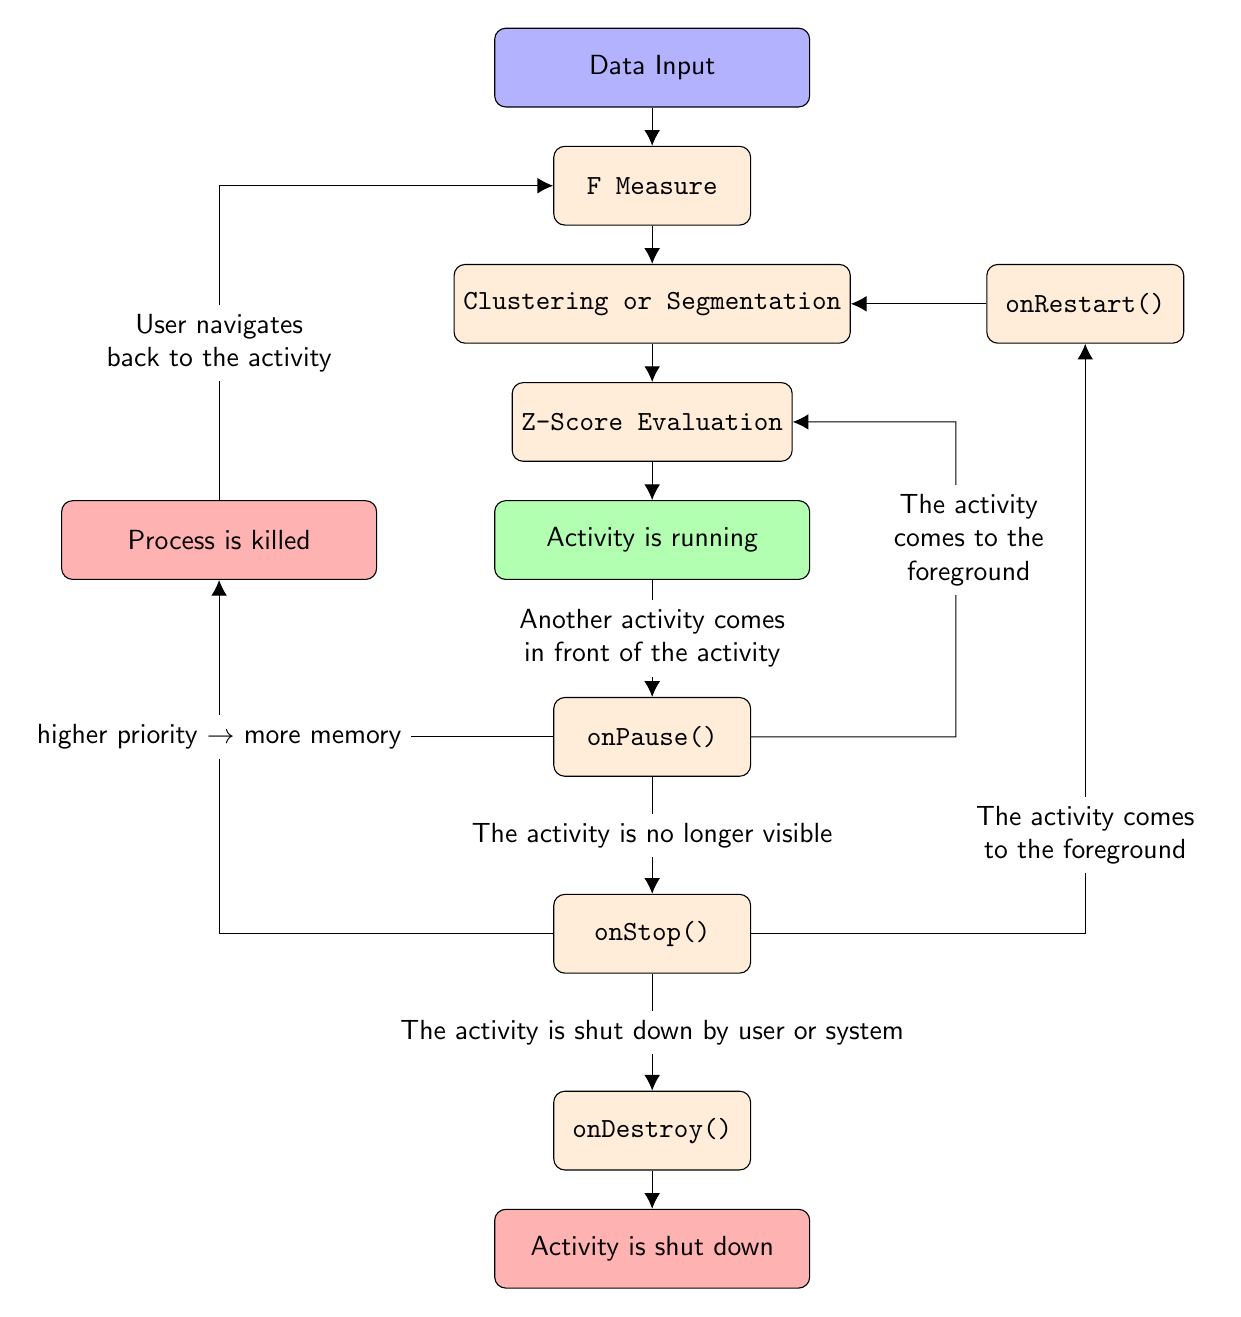
\begin{tikzpicture}[node distance=1.5cm,
    every node/.style={fill=white, font=\sffamily}, align=center]
  % Specification of nodes (position, etc.)
  \node (start)             [activityStarts]              {Data Input};
  \node (onCreateBlock)     [process, below of=start]          {F Measure};
  \node (onStartBlock)      [process, below of=onCreateBlock]   {Clustering or Segmentation};
  \node (onResumeBlock)     [process, below of=onStartBlock]   {Z-Score Evaluation};
  \node (activityRuns)      [activityRuns, below of=onResumeBlock]
                                                      {Activity is running};
  \node (onPauseBlock)      [process, below of=activityRuns, yshift=-1cm]
                                                                {onPause()};
  \node (onStopBlock)       [process, below of=onPauseBlock, yshift=-1cm]
                                                                 {onStop()};
  \node (onDestroyBlock)    [process, below of=onStopBlock, yshift=-1cm] 
                                                              {onDestroy()};
  \node (onRestartBlock)    [process, right of=onStartBlock, xshift=4cm]
                                                              {onRestart()};
  \node (ActivityEnds)      [startstop, left of=activityRuns, xshift=-4cm]
                                                        {Process is killed};
  \node (ActivityDestroyed) [startstop, below of=onDestroyBlock]
                                                    {Activity is shut down};     
  % Specification of lines between nodes specified above
  % with aditional nodes for description 
  \draw[->]             (start) -- (onCreateBlock);
  \draw[->]     (onCreateBlock) -- (onStartBlock);
  \draw[->]      (onStartBlock) -- (onResumeBlock);
  \draw[->]     (onResumeBlock) -- (activityRuns);
  \draw[->]      (activityRuns) -- node[text width=4cm]
                                   {Another activity comes in
                                    front of the activity} (onPauseBlock);
  \draw[->]      (onPauseBlock) -- node {The activity is no longer visible}
                                   (onStopBlock);
  \draw[->]       (onStopBlock) -- node {The activity is shut down by
                                   user or system} (onDestroyBlock);
  \draw[->]    (onRestartBlock) -- (onStartBlock);
  \draw[->]       (onStopBlock) -| node[yshift=1.25cm, text width=3cm]
                                   {The activity comes to the foreground}
                                   (onRestartBlock);
  \draw[->]    (onDestroyBlock) -- (ActivityDestroyed);
  \draw[->]      (onPauseBlock) -| node(priorityXMemory)
                                   {higher priority $\rightarrow$ more memory}
                                   (ActivityEnds);
  \draw           (onStopBlock) -| (priorityXMemory);
  \draw[->]     (ActivityEnds)  |- node [yshift=-2cm, text width=3.1cm]
                                    {User navigates back to the activity}
                                    (onCreateBlock);
  \draw[->] (onPauseBlock.east) -- ++(2.6,0) -- ++(0,2) -- ++(0,2) --                
     node[xshift=1.2cm,yshift=-1.5cm, text width=2.5cm]
     {The activity comes to the foreground}(onResumeBlock.east);
  \end{tikzpicture}


\section{Conclusion}

\newpage

\part{Conclusion}

\clearpage

\newpage

\begin{thebibliography}{}
\bibitem{WMG} 
Wei M, Gibbons LW, Mitchell TL \textit{et al}. (1999) The Association between cardiorespiratory fitness and impaired fasting glucose and type 2 diabetes mellitus in men. \textit{Ann Intern Med} \textbf{130}, 427-34.
\end{thebibliography}
\end{document}